\chapter{Вдоль Лысой горы на запад}

В этой главе мы пройдем вдоль Лысой горы («новой» Юрковицы) на запад, мимо юго-западного её склона, а в следующей, более обширной главе, обратимся ко склону восточному.

Прогулку, держа в уме, что двигаемся вдоль первоначального града Киева, начнем от перекрестка улицы Кирилловской (Фрунзе) и Нижнеюрковской (ранее части Юрковской, Большой Юрковской).

Южная сторона Лысой горы ограничена улицей Нижнеюрковской, сначала медленно, а потом круче поднимающейся в сторону Лукьяновки.

По левую руку от нас – Щекавица своим отрогом, где некоторые полагают Олегову могилу, а по правую руку будет Лысая гора, ныне частично спиленная. Прежде улица вписывалась бы в глубокий овраг, на плане 1752 года названный Унизовой долиной. Однако теперь северный берег ее на протяженности первых восьми номеров улицы попросту срыт.

На этой северной, четной стороне улицы сначала, у перекрестка с Кирилловской, по номеру 2, расположен кирпичный завод, затем  воинская часть, а над нею гаражный кооператив. Завода я еще коснусь, пока же скажу, что от него начинается ощутимый земляной вал, а сам завод и вч находятся на ровном плато у подножия горы.

Раньше этот огромный, поросший дикими травами пустырь покрывала часть горы, во второй половине 20 века срытая при добыче глины. Тогда и образовалось существующее поныне карьерное озеро, а в 1930-40 годах заполненные водой карьеры были на местах современного нам двора кирпичного завода да к востоку от военной части, от нее по общагу на Нижнеюрковской 4, включительно.

Вал идет вдоль всей воинской части, прерываясь у заезда на её территорию. С восточной стороны вал резко поворачивает на север в районе дома №4. Кстати всё, что сказано ниже об археологических находках в районе воинской части, с равным успехом можно отнести к соседнему с ней четвертому номеру. Четкой, до метров, привязки к местности у меня нет.

По отрывочным пересказам рукописи Е. В. Максимова, который проводил раскопки на Лысой горе в 1965 году, известно, что он обнаружил древний, 2-1 веков до нашей эры вал на «восточном склоне». 

Если под восточным склоном подразумевался срытый затем участок за кирпичным и пивным заводами, то вал на Нижнеюрковской может быть продолжением вала Максимова. Датировка последнего обосновывалась учеными керамикой, найденной в перекрытых валом ямах.

Примерно на месте современной воинской части, когда здесь была гора, Максимов нашел также остатки каркаса некой постройки с очагом и двумя горшками 10 века.

Викентий Хвойка зарисовал в своем дневнике вход в пещеру на склоне Лысой горы по нынешней улице Нижнеюрковской, вероятно, на уничтоженном участке холма. Где же подробности – описание пещеры? Неведомо. Но если уж Хвойка приложил усилия, чтобы зарисовать склон, значит, придавал пещере значение, а ведь эта картинка сама по себе малозначительна, содержимое пещеры куда ценнее!

\newpage
 
\begin{center}
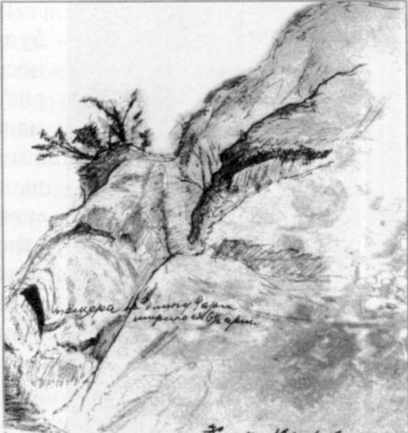
\includegraphics[width=\linewidth]{chast-kirvys/lys/hv-pesh.jpg}

\textit{Вход в пещеру на склоне. Рисунок Хвойки.}
\end{center} 

Позади военной части – заросший деревьями и кустами склон спускается к нижнему плато огромными террасами, образовавшимися от выемки глины.

Плато лежит за огражденной территорией кирпичного завода, завода солодовых экстрактов и пивзавода по улице Кирилловской (здания последних двух в 2014 выставлены на продажу). Возле склона, по соседству с полем на плато, в глубоком овраге прячется озеро, возникшее в карьере откуда добывали глину. Там водится рыба. Мне всегда было интересно, как рыба заводится в карьерных озерах. Благо, к этому озеру не добрались рыбаки.

\begin{center}
\includegraphics[width=\linewidth]{chast-kirvys/lys/\myimgprefix IMG_20130602_161845.jpg}

\textit{Карьерное озеро, 2013 год.}
\end{center} 

У срытой ныне южной стороны Лысой горы, примерно где военная часть, с 1816 года и по середину 19 века стоял, пожирая склон, кирпичный завод киевского гражданина Романовского\footnote{Завод был там и прежде, невесть с каких времен, просто Романовский купил завод в 1816-м.}, а позже – завод баронессы Фиркс\footnote{Адрес последнего в конце 19 века – Нижнеюрковская 4 и 6.}.

В этой местности, слывущей у старожилов поныне как Романовка или Романовщина, на задворках современной воинской части (Нижнеюрковская ул., 8а), под горкой, был пруд и оттуда вытекал ручей, который еще пару веков назад принято считать Юрковицей. Если идти по Нижнеюрковской снизу вверх, то дошагав по улице до конца воинской части, справа был бы этот овраг, а на месте самой воинской части – крутая гора. 

Современный коллектор, известный диггерам как коллектор ручья Юрковица – по длине больший, чем исторический ручей Юрковица. Коллектор принимает в себя более западные ручьи, которые несомненно впадали в Юрковицу и раньше. Вода в них очень студеная. Один из ручьев дренирован по склону на запад от котельной «Лукьяновской», напротив развалин дома 8-Б по Нижнеюрковской.

Последуем по Нижнеюрковской по мере нарастания номеров. Еще в 1980-90 годах тут, кроме прочего, стояли  выбеленные домики в один-два этажа, с деревянными пристройками, ставнями на окнах. Всё это снесено. Следы некоторых руин сохраняются в зарослях заброшенных фруктовых садов, у подножия горы по левую сторону. На месте прочих выбывших из строя зданий – заросшие пустыри, мусорники. Вот почему современная нумерация не сплошная, а с промежутками.

Что же сейчас? Дом номер 13 – типичная 9-этажная панельная гостинка с одним подъездом и сидячими ванными. Такие дома встречаются в Киеве всюду на обоих берегах. Напротив военной части, по адресу Нижнеюрковская, 5 – «Самостоятельная государственная пожарная часть №14 Подольского района». Идем дальше. Из канализационных люков под шоссе слышно журчание.

Дом номер 8-А – трехэтажный кирпичный жилой дом, старый добротный, во дворе своя котельная, и детская площадка – в такой глуши! Рядом, через кирпичную стену – руины тоже старого дома 8-Б\footnote{На 2021 год снесен, там новое здание.}, двухэтажного, с одноэтажной пристройкой и сараем. Судя по висящим внутри плакатам с гоночными автомобилями, люди обитали тут по крайней мере до 90-х. Пол внутри первого этажа загажен мусором. 

Если обойти дом, видно нечто вроде подпорной стены, а позади самого здания еще одна пристройка, где на втором этаже размещалось некое хозяйство – толстые окна из сине-зеленых плиток, дверь с обвалившимся крыльцом, на двери предупреждения не входить. Впрочем, за зелеными окнами нет ничего, всё внутри обрушено. Прогоревшая крыша заняла свободное пространство, а пол второго этажа исчез, вероятно упав на первый. Перед домом – кучи мусора.

Через улицу, напротив, под горой Юрковицей (исконной) – районная котельная «Лукьяновская» со здоровенной трубой (Нижнеюрковская 53). В первой половине 20 века всю котловину по нечетной стороне улицы занимали жилые дома.

Снова перейдем через дорогу к домам с номерами 8-А и 8-Б. От них справа, то есть на север, круто поднимается склон Лысой горы. Наверху расположился гаражный кооператив, вход куда строго охраняется. Чуть дальше по улице от дома 8-Б, направо – свалка под склоном, а налево – местность Чмелёва яра, до 1990-х застроенная очень старыми частными домами. 

Ее окрестности именовалась также Поляной. Вернее, было две Поляны, или Полянки – Старая и Новая. Первую называли еще, с начала 20 века, Антифеевкой. Мол, люди давали на лапу квартальному околоточному Антифееву и возводили здесь жилье.

Улица Старая Поляна – это часть давней улицы Чмелев яр. Другая сохранившаяся часть последней – современное окончание Лукьяновской от дома №11 вниз до Глубочицкой. Лукьяновская раньше шла прямо, никуда не заворачивая, и упиралась в улицу Чмелёв яр по месту теперешнего дома номер 9.

Очень малое количество старых частных домиков сохранилась выше, где Нижнеюрковская переходит в улицу Отто Шмидта, бывшую ранее частью улицы Юрковской. 

\newpage
\vspace*{\fill}
\begin{center}
\includegraphics[width=\linewidth]{chast-kirvys/lys/\myimgprefix IMG_4383.JPG}
\end{center} 

\begin{center}
\includegraphics[width=\linewidth]{chast-kirvys/lys/\myimgprefix IMG_4384.JPG}

\textit{2015 год. Домики в начале улицы Отто Шмидта.}
\end{center} 
\vspace*{\fill}
\newpage

Я не буду подробно пускаться в описание чехарды переименований, как от Юрковской отделили улицу Багговутовскую, после чего уже от нее отчекрыжили отрезок и назвали его Подлесной, да потом Большую Юрковскую поделили на Нижнеюрковскую и Верхнеюрковскую, а Верхнеюрковская вобрала Подлесную, а затем стала Отто Шмидта, но Багговутовская под разными вариантами названия то появлялась, то исчезала даже на дореволюционных картах, а в советское время стала улицей 9 января, однако победила Багговутовская.

Был такой генерал Александр Федорович Багговут (годы жизни 1806-1883), обитал примерно в этих краях на собственном хуторе\footnote{На 2020 год, хотя обнесенный строительным забором, сохраняется одноэтажный кирпичный домик дачи Багговутов, по адресу Багговутовская 16-18. По одной из версий считается, что именно тут одно время жили Праховы, и сюда к ним хаживал Врубель.} и был церковным старостой храма Федора Освященного, стараниями генерала и во многом на завещанные средства коллежского асессора Федора Иванова возведенного на углу Овручской и будущей Багговутовской.

Багговут с супругой слыли ярыми кладоискателями. Особо их привлекали места на Кирилловских высотах между Иорданской и Кирилловской церквями. Викентий Хвойка сетовал, что генерал «своими беспорядочными поисками» уничтожил «наиболее интересные в археологическом отношении места».

Итак, мы поднялись на уровень перекрестка\footnote{50°28'5.86"N 30°29'29.89"E}, поворота к гаражному кооперативу. Его северо-восточная часть выходит на дикий склон, что зарос деревьями и сплошь усеян битым, частью дореволюционным кирпичом. Следовательно, за теперешним кооперативом находились здания. Как давно их снесли и что там было – мне неведомо. Во всяком случае, на аэрофотоснимке 1943 года строений нет, пусто.

Остановлюсь у перекрестка да расскажу, что и где.

На юго-запад пошла узенькая улочка Старая Поляна. Заборы, машины, церковь-новодел, редкие пустыри, богатые терема. Ветхих, бедных домиков почти не сыщешь. По Старой Поляне можно выйти к лестнице на улицу Лукьяновскую. Нам не туда.

Вперед, на северо-запад, чешет дальше улица Отто Шмидта (с 1908 по 1917 он жил в доме №34, простоявшем до 1980-х).

К северо-востоку от упомянутого перекрестка находится безымянный переулок, идущий параллельно улице Отто Шмидта. Этот переулок служит межей жилого квартала (новые частные дома) и замусоренного обрыва с очень ровной границей. Местность сия именуется Романовкой, от того самого владельца кирпичного завода. Почти отвесный склон используется под свалку. Внизу его – широкая плоская местность на возвышенности, однако ниже, чем переулок. Она вся заросла большими деревьями, частью поваленными. В одном месте края обрыва есть дорожка, пологий спуск в сторону, на юго-восток. Дорожка огибает обрыв, постепенно сбавляя высоту и приближаясь к плато под ним.

Пройдя мимо него дальше по грунтовому спуску и свернув налево, к северо-востоку, мы попадаем на широчайшую часть склона, обращенного в сторону улицы Кирилловской и к самому нижнему плато, где территория кирпичного завода, завода солодовых экстрактов и озеро. Отсюда сверху видно всю Оболонь.

Склон сильно террасирован в том же направлении. Плоские уступы имеют ровные границы. Террасы эти возникли в ходе деятельности кирпичного завода – он просто сожрал часть склона Лысой горы, для добычи глины. Где-то здесь, напротив действующего еще в 2013 году «Пивзавода на Подоле», Антонович и нашел останки 2000 или 4000 людей, о чем я поведаю больше в следующей главе.

По всей этой части склона, кроме террас, видны старые следы других земляных работ – вероятно переходов между террасами, и еще чего-то. Например, в одном месте приходится идти по узенькой тропке, весьма приподнятой над остальным склоном – вот склон покатый, вот ниже тропка, и ниже тропки – резкий обрывчик. На дорожке между двумя уступами растут молодые сосенки.
 
Со стороны эта местность подобна стулу. Самая верхняя точка спинки – безымянный переулок, параллельный улице Отто Шмидта. Вниз – обрыв. Основное плато – сиденье стула. Далее там где ножки – уже террасы. У подножия – плато с полем и озером. Верхняя часть урочища именуется Романовщиной.

На террасах склона я не видел кирпичей. Россыпи их начались ближе к гаражному кооперативу. Непосредственный переход уступов к нижнему плато мною не изучен. Я был в 2013 году в разное время наверху, на нескольких террасах, ну и на нижнем пустыре возле озера. Всё это запечатлено на видео, когда мы снимали серии «Киевской амплитуды» – «Логово Змиево» и «Возвращение в Логово Змиево».
\vspace*{\fill}
\begin{center}
\includegraphics[width=0.95\linewidth]{chast-kirvys/lys/\myimgprefix IMG_20131026_160219.jpg}

\textit{2013. Вид с северо-восточного склона Лысой горы. Здание в центре – элеватор Пивзавода на Подоле, напротив ул. Кирилловской, 41 и 43.}
\end{center} 
\vspace*{\fill}
\newpage

На одном из верхних уступов мы нашли, кажется, остатки небольшого кладбища – ряд холмиков без опознавательных знаков. Я поначалу принял их за могилы, раскопанные в 1899-м археологом Беляшевским, но потом сообразил, что поскольку их разрыли, то ничего, кроме ям, не осталось бы, а тут холмики.

Вылезем снова на улицу Отто Шмидта. Если топать по ней дальше на северо-восток, то нас заинтересует первый же поворот. Сама улица сворачивает на запад, а вот на север отходит дорога в земли садового товарищества «Кожевник», лежащего на холме, соседнем с Лысой горой, к северо-западу от нее. 

Между Лысой и этим холмом – долгий овраг, по которому раньше была старая дорога на Лукьяновку от Иорданского монастыря, напоминающая въезд с подъемом в крепость. Сейчас там, по плоскому дну оврага дороги, сохранилась тропа\footnote{Верховье ее в декабре 2015 года перегородила частная усадьба.}, упирающаяся внизу в забор фабрики молочной кислоты (Кирилловская, 53) в бывшей усадьбе Марр. И если спуститься по дорожке и лестничке, мы попадаем в Иорданский переулок между фабрикой молочной кислоты (будет по левую руку) и нотной фабрикой справа. Идем вперед и попадаем на улицу Кирилловскую.
